\reading{MR-9}{Empirical Properties of Correlation: How Do Correlations Behave in the Real World?}{defer}{2}
% ==========================================================

\begin{mrkeybox}[title={Learning objectives in this reading}]
\small
\begin{enumerate}[label=\textbf{\alph*.},leftmargin=1.7em]
\item Describe how equity correlations and correlation volatilities behave throughout various
      economic states.
\item Identify the best-fit distribution for equity, bond, and default correlations.
\item Calculate a mean reversion rate using standard regression and calculate the corresponding
      autocorrelation.
\end{enumerate}
\end{mrkeybox}

\begin{mrtrapbox}[title={Note on ordering}]
The source notes present these as 8.a (economic states), 8.b (mean reversion) and 8.c
(distributions). The 2026 spine orders them \textbf{a} economic states, \textbf{b} best-fit
distribution, \textbf{c} mean reversion. The content below follows the spine.
\end{mrtrapbox}

% ---------------------------------------------------------
\lo{MR-9 a}{Describe how equity correlations and correlation volatilities behave throughout various economic states.}

\subsection{The study}
An empirical investigation analyzed correlations of the 30 common stocks in the Dow Jones
Industrial Average from 1972 to 2012.

\begin{itemize}
\item A $30 \times 30$ correlation matrix was created monthly, resulting in \term{426,300}
      monthly correlations after eliminating self-correlations.
\item Economic states were defined as \term{expansionary} (GDP $> 3.5\%$), \term{normal}
      ($0\% <$ GDP $\le 3.5\%$), and \term{recession} (two consecutive quarters of negative
      growth rates).
\item The study identified \term{six} recessions, \term{five} expansionary periods, and
      \term{five} normal periods within the analyzed timeframe.
\end{itemize}

\begin{center}
\small
\begin{tabular}{>{\raggedright\arraybackslash}p{5.0cm} r r}
\arrayrulecolor{FRMRule}\toprule
\rowcolor{FRMNavy} \hdr{State of the economy} & \hdr{Correlation level} & \hdr{Correlation volatility}\\
Expansionary period & 27.46\% & 71.17\%\\
\rowcolor{FRMSoft} Normal economic period & 33.06\% & \textbf{83.06\%} $\leftarrow$ highest\\
Recession & \textbf{36.96\%} $\leftarrow$ highest & 80.48\%\\
\bottomrule
\end{tabular}
\end{center}

\begin{center}
\begin{tikzpicture}
\begin{axis}[
  width=11.0cm, height=5.4cm,
  ybar=2pt, bar width=15pt,
  ymin=0, ymax=95,
  symbolic x coords={Expansion,Normal,Recession},
  xtick={Expansion,Normal,Recession},
  enlarge x limits=0.28,
  ylabel={\scriptsize Per cent},
  ylabel style={font=\scriptsize}, tick label style={font=\scriptsize},
  legend style={font=\scriptsize\sffamily, draw=FRMRule, fill=white,
    at={(0.5,-0.30)}, anchor=north, legend columns=-1, column sep=10pt},
  area legend,
  nodes near coords, nodes near coords style={font=\tiny\sffamily, color=black!70},
  every node near coord/.append style={/pgf/number format/fixed,
    /pgf/number format/precision=2},
  axis line style={draw=black!55}, clip=false]
\addplot[fill=PaleNavy, draw=FRMNavy!70, line width=0.4pt] coordinates {
(Expansion,27.46)(Normal,33.06)(Recession,36.96)};
\addlegendentry{Correlation level}
\addplot[fill=PaleRed, draw=FRMRed!70, line width=0.4pt] coordinates {
(Expansion,71.17)(Normal,83.06)(Recession,80.48)};
\addlegendentry{Correlation volatility}
\end{axis}
\end{tikzpicture}
\end{center}
\figcap{The two series do not peak in the same state, and that is the whole point of this
objective. The correlation \textit{level} rises steadily from expansion to recession. The
correlation \textit{volatility} peaks in the \textit{normal} period and then falls back slightly
in recession.}

\begin{mrtrapbox}[title={The counter-intuitive result}]
Surprisingly, the volatility was highest during the \term{normal} period rather than the
recession. This can be attributed to the increased uncertainty in a normal economy, where
investors are less certain about the overall direction of the stock market compared to
recessions or expansionary periods.
\end{mrtrapbox}

\begin{center}
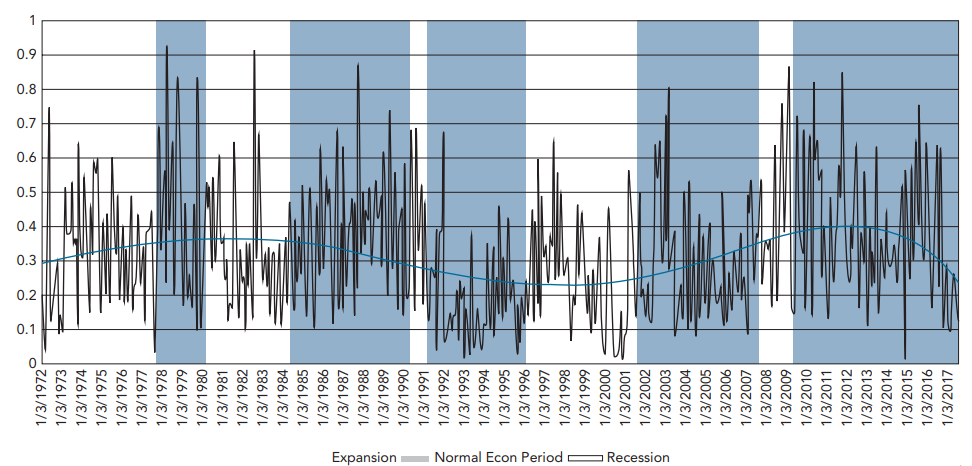
\includegraphics[width=0.94\linewidth]{fig/p87-004.png}
\end{center}
\figcap{Average correlation of the 30 Dow stocks, 1972 to 2017, with the shaded bands marking
economic states and the smooth line the trend. The jagged series is the monthly average; the
spikes cluster where the bands do.}

\begin{center}
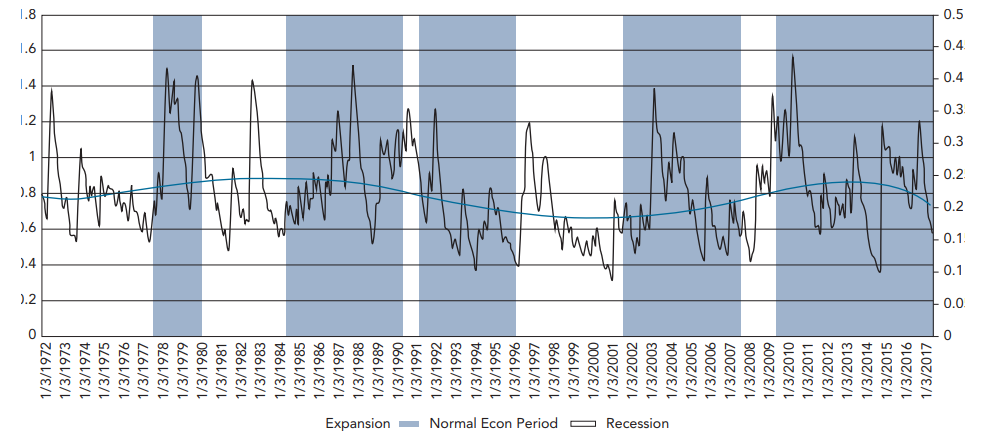
\includegraphics[width=0.94\linewidth]{fig/p88-004.png}
\end{center}
\figcap{The matching volatility series over the same period.}

% ---------------------------------------------------------
\lo{MR-9 b}{Identify the best-fit distribution for equity, bond, and default correlations.}

\subsection{Equity correlation distribution}
The input data of the distribution tests are daily correlation values between all 30 Dow stocks
from 1972 to 2017. This resulted in \term{464,580} correlation values. Most correlations between
the stocks in the Dow are positive: in fact, \term{77.23\%} of all 464,580 correlation values
were positive.

\begin{mrkeybox}[title={Findings of the fitting tests}]
\begin{itemize}
\item Three distribution fitting tests were used to determine the best fit for equity
      correlations.
\item The \term{Johnson SB} distribution --- which has two shape parameters, one location
      parameter, and one scale parameter --- provided the best fit for equity correlations.
\item The Johnson SB best fit was also \term{robust} with respect to testing different economic
      states for the time period in question.
\item The \term{normal, lognormal, and beta} distributions provided a \term{poor} fit for equity
      correlations.
\end{itemize}
\end{mrkeybox}

\begin{center}
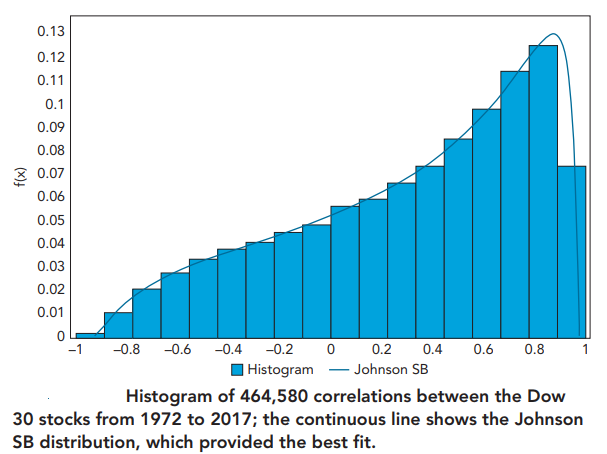
\includegraphics[width=0.72\linewidth]{fig/p93-004.png}
\end{center}
\figcap{The empirical distribution of the 464,580 daily Dow correlation values, with the fitted
curve. The mass sits to the right of zero, which is the 77.23\% positive figure seen as a shape.}

\subsection{Summary across the three correlation types}

\begin{center}
\small
\begin{tabular}{>{\raggedright\arraybackslash}p{3.3cm} r r r >{\raggedright\arraybackslash}p{3.1cm}}
\arrayrulecolor{FRMRule}\toprule
\rowcolor{FRMNavy} \hdr{Correlation type} & \hdr{Avg.\ corr.}
  & \hdr{Corr.\ vol.} & \hdr{Rev.\ rate} & \hdr{Best-fit distribution}\\
Equity & 35\% & 80\% & 78\% & Johnson SB\\
\rowcolor{FRMSoft} Bond & 42\% & 64\% & 26\% & Generalized Extreme Value\\
Default probability & 30\% & 88\% & 30\% & Johnson SB\\
\bottomrule
\end{tabular}
\end{center}
\figcap{Bond correlations are the highest on average but the least volatile and the slowest to
revert. Equity correlations revert fastest at 78\%. Two of the three are Johnson SB; bonds are
the odd one out.}

\begin{mrkeybox}[title={Note}]
For bond correlation data, the \term{normal} distribution would also have been a good fit
distribution.
\end{mrkeybox}

% ---------------------------------------------------------
\lo{MR-9 c}{Calculate a mean reversion rate using standard regression and calculate the corresponding autocorrelation.}

\begin{mrdefbox}[title={Mean reversion}]
Mean reversion is the tendency of a variable to be pulled back to its long-term mean. It implies
that over time, variables or returns regress back to the mean or average return. Statistically
it is defined as a \term{negative relationship} between the change in a variable over time and
the level of that variable. In finance, many variables --- bonds, interest rates, volatilities,
credit spreads and more --- are assumed to exhibit mean reversion.
\end{mrdefbox}

\begin{mrfmlbox}
\[ S_t - S_{t-1} \;=\; a\bigl( \mu - S_{t-1} \bigr)\Delta t \;+\; \sigma_S\,\epsilon\sqrt{\Delta t}
   \qquad\longrightarrow\qquad
   S_t - S_{t-1} \;=\; a\bigl( \mu - S_{t-1} \bigr) \]
\mrvk{$S_t$ = the value of the variable at time $t$;\quad $S_{t-1}$ = its value in the previous
period;\quad $\mu$ = the long-run mean;\quad $a$ = the \textit{mean reversion rate};\quad
$\sigma_S \epsilon \sqrt{\Delta t}$ = the stochastic term, which drops out when we take
expectations, leaving the deterministic form on the right.}{}
\end{mrfmlbox}

\subsection{Two rearrangements, for two different jobs}

\begin{center}
\small
\begin{tabularx}{\linewidth}{@{}p{6.6cm} >{\raggedright\arraybackslash}X@{}}
\arrayrulecolor{FRMRule}\toprule
\rowcolor{FRMNavy} \hdr{Form} & \hdr{Use it to}\\
$S_t = a(\mu - S_{t-1}) + S_{t-1}$
  & Calculate the \textbf{expected level} in the next period.\\
\rowcolor{FRMSoft}
$S_t - S_{t-1} = a\mu - a S_{t-1}$, matched term by term to $Y = \alpha + \beta X$
  & Calculate the \textbf{mean reversion rate} using regression.\\
\bottomrule
\end{tabularx}
\end{center}

\begin{center}
\begin{tikzpicture}[every node/.style={font=\small}]
  \node (lhs) at (0,0.9) {$S_t - S_{t-1}$};
  \node (eq) at (1.85,0.9) {$=$};
  \node (am) at (2.95,0.9) {$a\mu$};
  \node (mn) at (3.9,0.9) {$-$};
  \node (asx) at (5.15,0.9) {$a S_{t-1}$};
  \node[text=FRMGold] (Y) at (0,-0.55) {$Y$};
  \node[text=black] at (1.85,-0.55) {$=$};
  \node[text=FRMGold] (al) at (2.95,-0.55) {$\alpha$};
  \node[text=black] at (3.9,-0.55) {$+$};
  \node[text=FRMGold] (bx) at (5.15,-0.55) {$\beta X$};
  \foreach \a/\b in {lhs/Y, am/al, asx/bx}{
    \draw[FRMGold, -{Stealth[length=4pt]}, line width=0.8pt] (\a) -- (\b);}
  \node[anchor=west, font=\scriptsize\sffamily, text=black!65, text width=5.4cm]
    at (6.3,0.2) {so the regression \textbf{slope} is $-a$: a slope of $-0.78$ means a mean
    reversion rate of \textbf{78\%}};
\end{tikzpicture}
\end{center}
\figcap{The mapping is the whole trick. The change in the variable is the dependent variable,
the \textit{level} of the variable is the independent variable, and the mean reversion rate is
the slope with the sign flipped.}

\subsection{Calculating the mean reversion rate}
Standard regression analysis is one method used to estimate the mean reversion rate $a$. From
the 1972 to 2012 study, the data resulted in the following regression equation:
\[ Y \;=\; 0.27 - 0.78 X \]
The beta coefficient of $-0.78$ implies a mean reversion rate of \term{78\%}. This is a
relatively high mean reversion rate. Thus, if there is a large decrease (increase) from the mean
correlation for one month, the following month is expected to have a large increase (decrease)
in correlation.

\begin{mrexbox}[title={Example --- expected change at three different reversion rates}]
Suppose mean reversion exists for a variable with a value of 50 at time period $t-1$. The
long-run mean value $\mu$ is 80. What are the expected changes in value of the variable over the
next period, $S_t - S_{t-1}$, if the mean reversion rate $a$ is 0, 0.5, or 1.0?
\tcblower
\small
\begin{align*}
a = 0: \quad S_t - S_{t-1} &= 0 \times (80 - 50) = \mathbf{0} \quad \text{(no pull at all)}\\
a = 0.5: \quad S_t - S_{t-1} &= 0.5 \times (80 - 50) = \mathbf{15} \quad \text{(closes half the gap)}\\
a = 1.0: \quad S_t - S_{t-1} &= 1.0 \times (80 - 50) = \mathbf{30} \quad \text{(closes the whole gap in one step)}
\end{align*}
\end{mrexbox}

\begin{center}
\begin{tikzpicture}
\begin{axis}[
  width=10.6cm, height=5.7cm,
  xmin=-0.2, xmax=6.2, ymin=45, ymax=88,
  xlabel={\scriptsize Periods ahead}, ylabel={\scriptsize Value of $S$},
  xlabel style={font=\scriptsize}, ylabel style={font=\scriptsize},
  tick label style={font=\scriptsize},
  xtick={0,1,2,3,4,5,6}, ytick={50,60,70,80},
  legend style={font=\scriptsize\sffamily, draw=FRMRule, fill=white,
    at={(0.5,-0.30)}, anchor=north, legend columns=-1, column sep=10pt},
  axis line style={draw=black!55}, clip=false]
\addplot[FRMGold, dashed, line width=0.9pt, forget plot]
  coordinates {(-0.2,80)(6.2,80)};
\node[anchor=east, font=\scriptsize\sffamily, text=FRMGold] at (axis cs:6.1,83.5)
  {long-run mean $\mu = 80$};
\addplot[FRMRed, line width=1.1pt, mark=*, mark size=1.3pt]
  coordinates {(0,50)(1,50)(2,50)(3,50)(4,50)(5,50)(6,50)};
\addlegendentry{$a = 0$}
\addplot[FRMNavy, line width=1.1pt, mark=*, mark size=1.3pt]
  coordinates {(0,50)(1,65.0)(2,72.5)(3,76.25)(4,78.13)(5,79.06)(6,79.53)};
\addlegendentry{$a = 0.5$}
\addplot[FRMGreen, line width=1.1pt, mark=*, mark size=1.3pt]
  coordinates {(0,50)(1,80)(2,80)(3,80)(4,80)(5,80)(6,80)};
\addlegendentry{$a = 1.0$}
\end{axis}
\end{tikzpicture}
\end{center}
\figcap{The same starting point and the same mean, with only $a$ changing. At $a=0$ the variable
never moves; at $a=1$ it jumps straight to the mean and stays; at $a=0.5$ it halves the remaining
gap every period and approaches the mean asymptotically without ever quite arriving.}

\begin{mrexbox}[title={Example 1 --- calculating the expected correlation (solving for $S_t$)}]
In October 2012 the average monthly correlation for all Dow stocks was 30\% and the long-run
correlation mean of Dow stocks was 35\%. A risk manager runs a regression and the output
estimates $Y = 0.273 - 0.78X$. What is the expected correlation for November 2012?
\tcblower
\small
The slope of $-0.78$ gives a mean reversion rate of $a = 0.78$.
\begin{align*}
S_t - S_{t-1} &= a(\mu - S_{t-1}) = 0.78 \times (0.35 - 0.30) = 0.039\\
S_t &= 0.30 + 0.039 = \mathbf{0.339 \text{, or } 33.9\%}
\end{align*}
The correlation is pulled up from 30\% toward the 35\% mean, closing 78\% of the 5-point gap.
\end{mrexbox}

\begin{mrexbox}[title={Example 2 --- calculating the mean reversion rate}]
If correlations are now at 35\%, the long-term average of correlations is 0.45, and in the
previous year correlations were as low as 0.22, what is the mean reversion rate?
\tcblower
\small
Rearranging $S_t - S_{t-1} = a(\mu - S_{t-1})$ for $a$:
\[ a \;=\; \frac{S_t - S_{t-1}}{\mu - S_{t-1}} \;=\; \frac{0.35 - 0.22}{0.45 - 0.22}
   \;=\; \frac{0.13}{0.23} \;=\; \mathbf{0.5652 \text{, or } 56.52\%} \]
\end{mrexbox}

\subsection{Autocorrelation}
Autocorrelation is the degree to which a variable is correlated to its \term{past values}. It is
often calculated using an ARCH or GARCH model; an alternative approach is running a regression
equation.

\begin{mrdefbox}[title={The reverse property}]
Autocorrelation is the \term{``reverse property''} to mean reversion. The stronger the mean
reversion --- the more strongly a variable is pulled back to its long-term mean --- the
\term{lower} the autocorrelation, and vice versa.
\end{mrdefbox}

\begin{mrfmlbox}
\[ AC\bigl(\rho_t, \rho_{t-1}\bigr) \;=\;
   \frac{\mathrm{cov}\bigl(\rho_t, \rho_{t-1}\bigr)}{\sigma(\rho_t) \times \sigma(\rho_{t-1})}
   \qquad\qquad
   \text{Autocorrelation} \;=\; 1 - \text{mean reversion rate} \]
\mrvk{$\rho_t$ = the correlation value this period;\quad $\rho_{t-1}$ = the same variable one
period lagged. The right-hand shortcut only applies to the \textit{one-period lag}
autocorrelation.}{}
\end{mrfmlbox}

This autocorrelation equation was used to calculate the one-period lag autocorrelation of Dow
stocks for the 1972 to 2012 period, and the result was \term{22\%}, which is identical to
subtracting the mean reversion rate from one. Equivalently, a mean reversion of 77.51\% implies
an autocorrelation of 22.49\% --- the two add up to 1.

\begin{center}
\begin{tikzpicture}[every node/.style={font=\scriptsize\sffamily}]
  \fill[PaleNavy, draw=FRMNavy!60, line width=0.7pt] (0,0) rectangle (8.58,0.75);
  \fill[PaleGold, draw=FRMGold!70, line width=0.7pt] (8.58,0) rectangle (11.0,0.75);
  \node[text=FRMNavy] at (4.29,0.375) {\textbf{mean reversion  78\%}};
  \node[text=FRMGold] at (9.79,0.375) {\textbf{AC  22\%}};
  \draw[black!55, {Stealth[length=4pt]}-{Stealth[length=4pt]}, line width=0.5pt]
    (0,-0.32) -- (11.0,-0.32);
  \node[anchor=north, text=black!60] at (5.5,-0.36) {always sums to 1};
\end{tikzpicture}
\end{center}
\figcap{The two are complements of each other, so being given either one hands you the other
immediately. This is a standard one-line exam item.}


% ==========================================================
